\section{Normalizing Flows}


For a \textbf{univariate} case, 
\begin{itemize}
    \item $Z$: source random variable and density $p(z)$
    \item $X$: target random variable and density $q(x)$
    $$T: Z\rightarrow X$$
    \item  
    $$q(x) = p(z)\Big|\frac{\partial T(z)}{\partial z}\Big|^{-1}$$
\end{itemize}

For a \textbf{multivariate} case
$$\mathbf{T}: \mathbb{R}^d \rightarrow \mathbb{R}^d$$
So, 
$$q(\mathbf{x})= p(\mathbf{x})|\det \nabla_{\mathbf{z}}\mathbf{T}(\mathbf{z})|^{-1}$$

For example,
\begin{itemize}
    \item  $\mathbf{X}\in \mathbb{R}^d$ and $\mathbf{Z}\in \mathbb{R}^d$
    \item  $\mathbf{X} = (\mathbf{x}_1, ..., \mathbf{x}_d)$ and $\mathbf{Z} = (\mathbf{z}_1, ..., \mathbf{z}_d)$
    \item $\mathbf{T} = (T_1, T_2,...,T_d)$
    \item $\mathbf{x}_1 = T_1(\mathbf{z})$, $\mathbf{x}_2 = T_2(\mathbf{z})$, $\mathbf{x}_d = T_d(\mathbf{z})$
\end{itemize}

Jacobian matrix of $\mathbf{T}$ is given by
\begin{align*}
 \nabla_{\mathbf{z}}\mathbf{T}(\mathbf{z})  = \begin{bmatrix}
    \frac{\partial T_1}{\partial z_1} &\frac{\partial T_1}{\partial z_2} &\cdots &\frac{\partial T_1}{\partial z_d} \\
    \frac{\partial T_2}{\partial z_1} &\frac{\partial T_2}{\partial z_2} &\cdots &\frac{\partial T_2}{\partial z_d} \\
    \vdots& \vdots &\ddots &\vdots\\
    \frac{\partial T_d}{\partial z_1} &\frac{\partial T_d}{\partial z_2} &\cdots &\frac{\partial T_d}{\partial z_d} 
 \end{bmatrix}
\end{align*}

Our goal is to estimate the dataset $\mathcal{D} = \{\mathbf{x}_1, ..., \mathbf{x}_n\}\sim q(\mathbf{x})$

\begin{itemize}
    \item Choose a simple density $p(z)$
	\item We want to estimate $q(\mathbf{x})$ by using MLE:
    \begin{align*}
        \prod_{i=1}^{n}q(\mathbf{x}_i) &= \prod_{i=1}^{n}p(\mathbf{z}_i)|\det \nabla_{\mathbf{z}}\mathbf{T}(\mathbf{z})|^{-1} \quad \textrm{by change of variable}\\
        \hat{\mathbf{T}} &:= \argmax_{\mathbf{T}}\prod_{i=1}^{n} p(\mathbf{z}_i)|\det \nabla_{\mathbf{z}}\mathbf{T}(\mathbf{z})|^{-1}\\
        \hat{\mathbf{T}} &:= \argmax_{\mathbf{T}}\sum_{i=1}^{n} \log p(\mathbf{z}_i) - \log |\det \nabla_{\mathbf{z}}\mathbf{T}(\mathbf{z})|
    \end{align*}
    \item $\mathbf{z}_i = \mathbf{T}^{-1}(\mathbf{x}_i)$
    \item We need to compute the inverse $\mathbf{T}^{-1}$, which is computationally expensive
    \item We want to avoid the issue by using Jacobian trainagular matrix 
\end{itemize}

\subsection{Triangular Maps}
$$\mathbf{T}: \mathbb{R}^d \rightarrow \mathbb{R}^d$$
\begin{align*}
    \nabla_{\mathbf{z}}\mathbf{T}(\mathbf{z})  = \begin{bmatrix}
    \frac{\partial T_1}{\partial z_1} & 0 &\cdots & 0\\
    \frac{\partial T_2}{\partial z_1} &\frac{\partial T_2}{\partial z_2} &\cdots & 0\\
    \vdots& \vdots &\ddots &\vdots\\
    \frac{\partial T_d}{\partial z_1} &\frac{\partial T_d}{\partial z_2} &\cdots &\frac{\partial T_d}{\partial z_d} 
 \end{bmatrix}
\end{align*}
Increasing: $T_j$ is w.r.t $z_j$. Determinant is the product of diagonal elements.
\begin{itemize}
    \item $x_1 = T_1(z_1)$
    \item $x_2 = T_2(z_1, z_2)$
    \item $x_3 = T_2(z_1, z_2, z_3)$
    \item $x_d = T_2(z_1, z_2, ..., z_d)$
\end{itemize}
\begin{align*}
    \min_{\mathbf{T}}\sum_{i=1}^{n} \Bigg[-\log p(\mathbf{T}^{-1}(\mathbf{x}_i)) + \sum_{j}\log \frac{\partial T_j}{\partial z_j}\Bigg] 
\end{align*}

\begin{figure}[t]
	\centering
	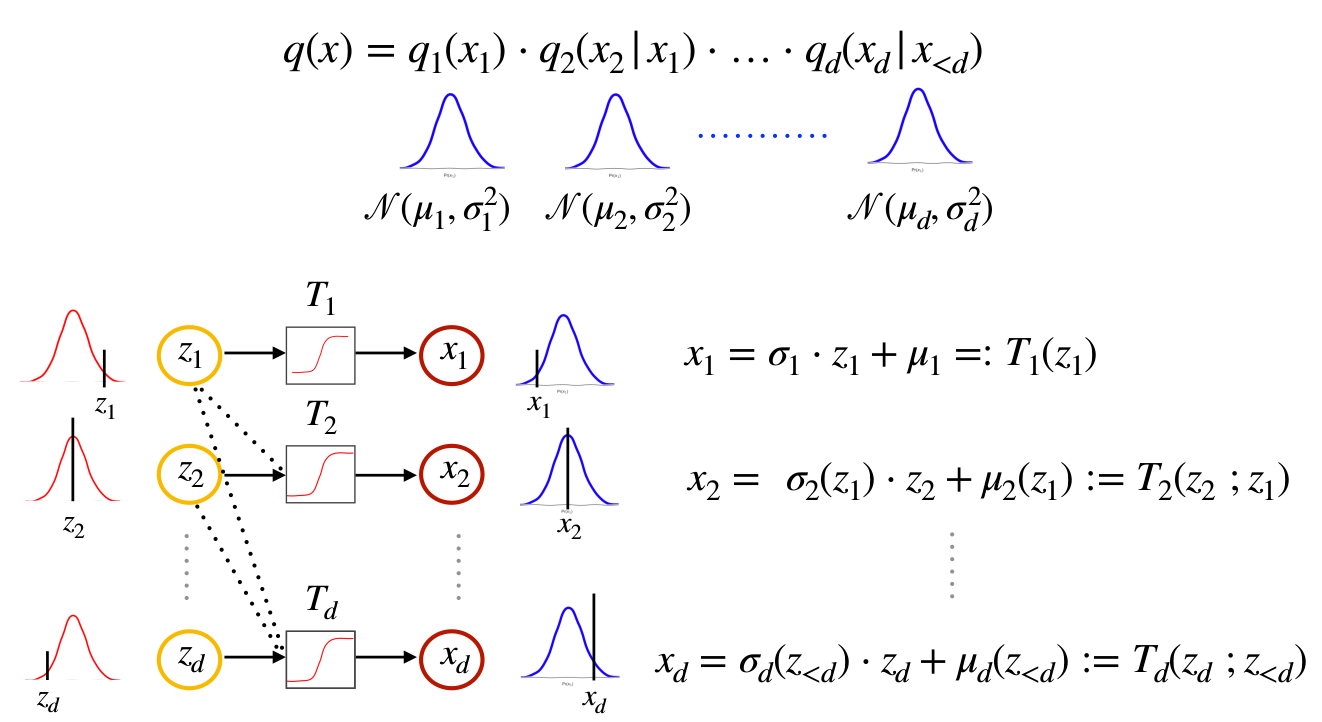
\includegraphics[scale=0.30]{./images/generative/flows/nmf.png}
\end{figure}
